\section{\secquant}
\label{sec_quant_cex}

In \Cref{act_TorF} there were statements involving variables in which the truth of the statement depended on whether the statement was about all values, some values, or no values of the variables.  Each of the words ``all'', ``some'', and ``no'' has a specific meaning in mathematics and computer science.  In this section, we consider such \vocab{quantifiers} and their negations and formally introduce the idea of a \vocab{counterexample}.  We also look at how to prove quantified statements.

%%%%%%%%%%%%%%%%%%%%%%%

\newcommand{\subsetgame}{The Game SET}
\subsection{\subsetgame}
\label{sub_set_game}

Let's start with a puzzle.

The game SET\texttrademark~ is produced by SET Enterprises, part of Monster Play.  You can learn to play the game at \url{https://tinyurl.com/learntoplaySET}.  There is a lot of information about this game on the Internet. Resist the temptation to use any resources to find answers to this (or any) activity.  The fun part is figuring it out for yourself! 

\begin{act}[The game SET\texttrademark]
\label{act_set_game}
    In the game SET\texttrademark, there is a deck of special cards. Each card has the image of some number of a colored shape with some level of shading. If there is more than one shape on a card, the others shapes on the card are repeats of that shape with the same color and level of shading.  For example, there is a card that has two striped, purple ovals, as shown in \Cref{fig_SET_2SPO}.
        \begin{figure}[hbtp]
            \centering
            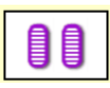
\includegraphics[scale=.5]{Images/2SPO.png}
            \caption{The SET\texttrademark ~ card with two striped, purple ovals. (\textbf{2SPO)}}
            \label{fig_SET_2SPO}
        \end{figure} 
    
    There are four characteristic of the image on each card: number, shading, color, and shape. Each characteristic has three options as summarized in \Cref{table_set_game_card_options}. 
    
        \begin{table}[hbtp]
            \centering
            \begin{tabular}{l|l}
                characteristic & options (with their abbreviations) \\ \hline
                number & \textbf{1}, \textbf{2}, or \textbf{3} \\ 
                shading & none (\textbf{N}), striped (\textbf{S}), or full (\textbf{F})\\
                color &  red (\textbf{R}), purple (\textbf{P}), or green (\textbf{G}) \\ 
                symbol & oval (\textbf{O}), diamond (\textbf{D}), or squiggle (\textbf{Q}) 
            \end{tabular}
            \caption{The options for each characteristic for the image on each card in the game SET\texttrademark.}
            \label{table_set_game_card_options}
        \end{table}

    \begin{actpart}
        \item Write the abbreviation for each card shown in \Cref{figure_set_game_2cards}.  The card on the left is green and the card on the right is red.
            \begin{figure} [hbtp]
                \centering
                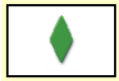
\includegraphics[scale=.5]
                {Images/1FGD} \quad
                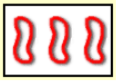
\includegraphics[scale=.5]{Images/3NRQ} 
                \caption{Two cards from the game SET\texttrademark.}
                \label{figure_set_game_2cards}
            \end{figure}
            
        \item For each combination of options there is exactly one card in the deck with that combination. How many cards are there in the game SET\texttrademark? Explain.
        
        \item A set of three cards is a \vocab{SET} if for each of the characteristics either the images on the three cards all agree or are all different.  That is, all four of the following conditions must be met.
            \begin{bull}
                \item All three cards have the same number or there is one with 1, one with 2, and one with 3.  
                \item All three cards have the same shading or there is one with none, one striped, and one full.  
                \item All three cards have the same color or there is one red, one purple, and one green.
                \item All three cards have the same symbol or there is one oval, one diamond, and one squiggle. 
           \end{bull}
        Check that the set of three cards shown in \Cref{figure_show_set} is a SET.  
            \begin{figure}[hbtp]
                \centering
                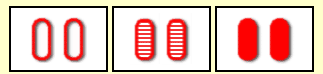
\includegraphics[scale=.5]{Images/IsSET}
                
                \{\textbf{2NRO}, \textbf{2SRO}, \textbf{2FRO}\}
                \caption{An example of a SET.}
                \label{figure_show_set}
            \end{figure}
            
        \item Is the set of three cards shown in \Cref{figure_decide_if_set} a SET? Justify your answer.
            \begin{figure}[hbtp]
                \centering
                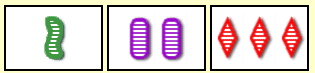
\includegraphics[scale=.5]{Images/AnotherSET}
                
                \{\textbf{1SGQ}, \textbf{2SPO}, \textbf{3SRD}\}
                \caption{Is this set of three cards a SET?}
                \label{figure_decide_if_set}
            \end{figure}
            
        \item Explain why the set of three cards shown in \Cref{figure_show_not_set} is not a SET.
            \begin{figure}[hbtp]
                \centering
                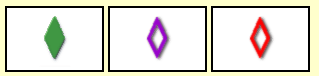
\includegraphics[scale=.5]{Images/NotSET}

                \{\textbf{1FGD}, \textbf{1NPD}, \textbf{1NRD}\}
                \caption{An example of three cards that are not a SET.}
                \label{figure_show_not_set}
            \end{figure}
            
        \item Is the set of three cards shown in \Cref{figure_all_diff_set} a SET? Justify your answer.
            \begin{figure}[hbtp]
                \centering
                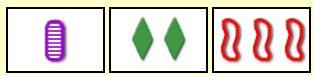
\includegraphics[scale=.5]{Images/AllDiffSET}

                \{\textbf{1SPO}, \textbf{2FGD}, \textbf{3NRQ}\}
                \caption{Is this different set of three cards a SET?}
                \label{figure_all_diff_set}
            \end{figure}

        \item What third card makes a SET with the pair of cards from \Cref{figure_set_game_2cards}?

        \item Given a pair of cards, explain how we can find a third card that makes a SET with the given pair. Be sure to explain in general (tell someone step-by-step how to find the missing third card.) 
    \end{actpart}
\end{act}
 
%%%%%%%%%%%%%%%%%%%%%%%%%%%%%%%%%%%%%%%%%%
\newcommand{\subquant}{Quantifiers}
\subsection{\subquant}
\label{sub_quantifiers}

In the game SET\texttrademark, a set of three cards forms a SET if for each characteristic, all the cards agree or none of the cards agree.  A set of three cards is not a SET if, for some characteristic, the cards have two of one kind and one of a different kind. Part of the challenge of learning the game is grappling with words like ``each'', ``all'', ``none'', and ``some'' which are examples of quantifiers.

\begin{defn}[Quantifiers]
\label{defn_quantifiers}
    Quantifiers can be defined on any set.  Throughout this definition, our examples use the set of integers.
    \begin{apart}
        \item We indicate that a statement $P$ depends on a variable $n$ by writing $P(n)$ instead of $P$.  The notation $P(n)$ is \vocab{predicate notation}.  For example, if $P(n)$ means that the integer $n$ is odd, then $P(3)$ means that the integer $3$ is odd, which is true, but $P(10)$ means that the integer $10$ is odd, which is false. 

        \item The \vocab{universal quantifier}, denoted $\forall$, means ``for all''. 
            \begin{bull}             
                \item The statement $\forall n P(n)$ means that
                    \begin{center}
                        $P(n)$ is true for all values of $n$.
                    \end{center} 
                For example, if $P(n)$ means that the integer $2n$ is even, then $\forall n ~ P(n)$ means that every integer of the form $2n$ is even,
                which is true.  On the other hand, if $Q(n)$ means that $3 \mid n$, then $\forall n ~ Q(n)$ means that every integer is divisible by three, which is false because, for example, 17 is not divisible by three.
                \item The statement $\forall n(\neg P(n))$ means
                    \begin{center}
                        $P(n)$ is false for all values of $n$.           
                    \end{center}
                For example, if $R(n)$ means that the integer $2n+1$ is even, then $\forall n (\neg R(n))$ means that no integer of the form $2n+1$ is even, which is true.
            \end{bull}
        
        \item The \vocab{existential quantifier}, denoted $\exists$ means ``there exists.'' 
            \begin{bull}
                \item The statement $\exists n ~ P(n)$ means that
                    \begin{center}
                        $P(n)$ is true for some value(s) of $n$. 
                    \end{center} 
                For example, if $Q(n)$ means that $3 \mid n$, then $\exists n ~ Q(n)$ means that some integer is divisible by three, which is true because, for example, 12 is divisible by three.  
                \item The statement $\exists n (\neg P(n))$ means that
                    \begin{center}
                        $P(n)$ is false for some value(s) of $n$. 
                    \end{center} 
                For example, if $Q(n)$ means $3 \mid n$, then $\exists n (\neg Q(n))$ means that some integer is not divisible by three, which is true because, for example, 17 is not divisible by three.
            \end{bull}
    \end{apart}
\end{defn}

There are many different English words and phrases that indicate quantifiers.

\begin{rem}[English words indicating quantifiers]
~
    \begin{apart}
        \item Words and phrases that indicate a universal quantifier include: 
            \begin{center}
                a, all, always, any, each, every, everyone, etc.
            \end{center}
        \item Words and phrases that indicate a universal quantifier followed by a negation include: 
            \begin{center}
                impossible, never, no, no one, none, nothing, etc.
            \end{center}
        \item Words and phrases that indicate an existential quantifier include: 
            \begin{center}
                at least one, can, contains, has, possible, some, someone,\\ sometimes, there exist, there exists there is, there are, etc.
            \end{center}
        \item Note that some words and phrases that indicate the existential quantifier are plural, but it takes only one value of $n$ where $S(n)$ is true to make the statement $\exists n ~ S(n)$ true.  For example, in mathematics, some means at least one.
    \end{apart}
\end{rem}

Universally quantified statements are sometimes written without an explicit quantifier.  For example, we might say $2n$ is even when we really mean $2n$ is even for all integers $n$.

\begin{rem}[Default universal]
\label{rem_default_universal} 
    If a statement about variables does not explicitly state a quantifier, the default assumption is that the quantifier is universal.  
\end{rem}

Practice working with quantified statements.

\begin{act}[More true or false?]
\label{act_TorF_again}
    Identify a word or phrase that indicates a quantifier, decide if each statement is true or false, and discuss how to justify your answer. 
        \begin{actpart}
            \item \label{part_exists_5vert_5edge} There is a graph that has five vertices and five edges. % exists True
            \item \label{part_forall_5vert_5edge} Any graph with five vertices has five edges.% for all exists False
            \item \label{part_more_edges_than_verts} No graph has more edges than vertices. %False NO EXISTS 
            \item \label{part_sq_has3div} Some square integers have exactly three positive divisors. %True EXISTS EXISTS
            \item \label{part_sq_ex3div} Any square integer has exactly three positive divisors. %False FOR ALL EXISTS 
            \item \label{part_regular_graph} Some graphs are regular.  Recall that in a \vocab{regular} graph, every vertex has the same degree. %True  EXISTS FOR ALL 
            \item \label{part_not_regular_graphs} Some graphs are not regular. % True Exists not all
        \end{actpart}
\end{act}

Let's look at a few more examples identifying words or phrases that indicate a quantifier.

\begin{exam}[Identifying quantifiers]
\label{exam_words_quants}
    In each statement, find a word or phrase that indicates a quantifier and say which: $\forall$ or $\exists$.  In some parts, both quantifiers are involved.  (We saw these statements in \Cref{act_TorF} and \Cref{act_TorF_again}.)
        \begin{apart}
            \item  There are three distinct digits whose sum is 23.
                \begin{soln}
                    The phrase ``there are'' indicates an existential quantifier $\exists$.
                \end{soln}

            \item Some integers are divisible by three and five.
                \begin{soln}
                    The word ``some'' indicates an existential quantifier $\exists$.
                \end{soln}
                
            \item A graph with five vertices is the cycle $C_5$ or the complete graph $K_5$. 
                \begin{soln}
                    The word ``a'' indicates a universal quantifier $\forall$.
                \end{soln}
                
            \item  
            No graph has more edges than vertices. 
                \begin{soln}
                    The word ``no'' indicates a universal quantifier $\forall$.
                \end{soln}
                
            \item \label{part_bs5_contains1} Every bit string of length five contains at least one \bs{1}.
                \begin{soln}
                    The word ``every'' indicates a universal quantifier $\forall$ and the word ``contains'' indicates an existential quantifier $\exists$.
                \end{soln}
        \end{apart}
\end{exam}

%%%%%%%%%%%%%%%%%%%%%%%%%%%%%%%%%%%%%%%%%%
\newcommand{\subpffquants}{Proof Formats: $\forall$ and $\exists$}
\subsection{\subpffquants}
\label{sub_pff_quants}

How do we prove that a quantified statement is true?

To prove an existentially quantified statement, all we need to do is provide an example.  Here is the proof format.

\begin{pff}[Existentially-quantified statements]
\label{pff_exists}  
    Prove: $\exists n ~ P(n)$.

    \begin{proof} Consider $n=$ (example).\\
    (Explain why $P(n)$ is true.)\\
    Therefore, $P(n)$ is true for some (describe type of object) $n$, namely $n=$ (example).       
    \end{proof}
\end{pff}

In the first sentence of \Cref{pff_exists} we present an example without any explanation of how we found that example.  Mathematicians sometimes explain where the example came from, but that explanation is not a required part of the proof.  Let's look at a quick example.

\begin{exam}[There is a graph with five vertices and five edges]
\label{exam_exists_graph_5vert_5edge}
    Prove \Cref{act_TorF_again} (\ref{part_exists_5vert_5edge}) that there is a graph that has five vertices and five edges.
        \begin{soln}
            The phrase ``there is'' indicates an existentially quantified statement, so we follow \Cref{pff_exists}.
            
                \emph{Proof.} 
                    Consider the cycle $C_5$.  Recall that $C_5$ has five vertices and five edges.  Therefore, there is a graph that has five vertices and five edges, namely $C_5$.     
        \end{soln}
\end{exam}

The proof of a universally quantified statement is more complicated because we have to prove that the statement holds for all possible examples.  In some cases, we can simply check every example.

\begin{exam}[Checking every example]
\label{exam_check_every_example}
    In \Cref{sec_mod_arith}, we introduced the integers mod 5, $\mathbb{Z}_5=\{0,1,2,3,4\}$. In $\mathbb{Z}_5$, 
    %addition is defined by $a \oplus b = a+b \fn{ mod } 5$ and 
    multiplication is defined by $a \otimes b = ab \fn{ mod } 5$.
    Prove that there is no solution to $x^2=2$ in $\mathbb{Z}_5$.  Note that $x^2 = x \otimes x$.
        \begin{soln}
            We can check each element of $\mathbb{Z}_5$ to see if it is a solution. Our work is displayed in \Cref{tab_dne_sqrt2_mod5}. Since none of the elements of $\mathbb{Z}_5$ is a solution, we can conclude that there is no solution to $x^2=2$ in $\mathbb{Z}_5$.
                \begin{table}[hbtp]
                    \centering
                    \begin{tabular}{c|c|c}
                        $x$ & evaluate $x^2$ in $\mathbb{Z}_5$ & does $x^2=2$? \\ \hline
                        0 & $0^2 = 0\fn{ mod } 5= 0$ & no \\ \hline
                        1 & $1^2 = 1\fn{ mod } 5= 1$ & no \\ \hline
                        2 & $2^2 = 4\fn{ mod } 5= 4$ & no \\ \hline
                        3 & $3^2 = 9\fn{ mod } 5= 4$ & no \\ \hline
                        4 & $4^2 = 16\fn{ mod } 5= 1$ & no 
                    \end{tabular}
                    \caption{Checking that $x^2=2$ has no solution in $\mathbb{Z}_5$.}
                    \label{tab_dne_sqrt2_mod5}
                \end{table}
        \end{soln}   
\end{exam}

In the previous example, we were able to check all five possible examples.  But if the list of possible examples is very long or infinite, it is not reasonable or possible to check every example, and it is not enough to just check some examples.  Here is the proof format.

\begin{pff}[Universally-quantified statements]
\label{pff_forall}  
    Prove: $\forall n ~ P(n)$.

    \begin{proof} Let $n$ be an (describe the type of object). \\
    (Explain why $P(n)$ is true.)  \\
    Therefore, $P(n)$ is true for all (describe the type of object) $n$.       
    \end{proof}
\end{pff}

The proof begins by naming an arbitrary object, $n$, of the type described. This first sentence invites the reader to select any value of $n$.  Next, we show that the statement is true for that particular but unknown $n$. Our proof must work for whatever value $n$ the reader selected.

Let's look at a quick example.

\begin{exam}[$6q-10$ is even]
\label{exam_6qminus10_is_even}
    Use the definition of even to prove that for every integer $q$, the integer $6q-10$ is even.  (This proof was \Cref{sec_even_odd_divides} \Cref{exer_linears_even_odd} (\ref{part_6qminus10_is_even}).)
        \begin{soln}
            The phrase ``for every'' indicates a universally quantified statement, so we follow \Cref{pff_forall}.
        
                \emph{Proof.} 
                    Let $q$ be an integer. Then $6q-10=2(3q-5)=2k$ where $k=3q-5$ is an integer.  By the definition of even, it follows that $6q-10$ is even. Therefore, for every integer $q$, the integer $6q-10$ is even.  
        \end{soln}
\end{exam}

As usual, after we introduce new proof formats, we give you the opportunity to practice.

\begin{act}[Proofs of quantified statements]
\label{act_proof_quants}  
~
    \begin{actpart}
        \item \label{part_exists_int_4div} Copy the following proof. Note that the phrase ``there is'' indicates an existentially quantified statement, so we use \Cref{pff_exists}.

        Prove that there is an integer that has exactly four positive divisors.  
            \begin{proof}
                Consider the integer six.  The positive divisors of six are 1, 2, 3, and 6.  Thus, six has exactly four positive divisors. Therefore, there is an integer that has exactly four positive divisors.
            \end{proof}
        
        \item Edit the proof in (\ref{part_exists_int_4div}) to prove that there is an integer with exactly three positive divisors.
        \item \label{part_ndivnfactorial} Copy the following proof. Note that the phrase ``for any'' indicates a universally quantified statement, so we use \Cref{pff_forall}.

        Prove $n \mid n!$ for any integer $n$. 
            \begin{proof}
                Let $n$ be an integer.  Note that $n!=n(n-1)!=nk$ where $k=(n-1)!$  By the definition of divides, it follows that $n \mid n!$ Therefore, $n \mid n!$ for every integer $n$.
            \end{proof}
        \item Edit the proof in (\ref{part_ndivnfactorial}) to prove $2 \mid 2^n$ for any integer $n$.
    \end{actpart}
\end{act}

Many interesting mathematical statements involve both existential and universal quantifiers.  Fortunately, we do not need new proof formats.  Instead, we can nest proof formats one inside the other, as if they were Matryoshka dolls\footnote{See wikipedia Matryoshka doll.} or nested loops in computer programming.  Try writing proofs that nest the proof formats for existentially and universally quantified statements.

\begin{act}[Proofs of nested quantified statements]
\label{act_proof_quants_nested} 
~
    \begin{actpart}
        \item \label{part_proof_forall_exists} Copy the following proof. Note that we use \Cref{pff_forall} and, within that format, we use \Cref{pff_exists}. We have indented the lines to highlight the nesting.

        Prove that for any integer $n$ there is an integer $m$ such that $n+m=100.$
        
            \begin{proof}
                Let $n$ be an integer.  
                
                \hspace{.75in} Consider the integer $m=100-n$. 
                
                \hspace{.75in}\hspace{.75in} Then $n+m=n+(100-n)=100.$ 
                
                \hspace{.75in} Thus, there is an integer $m$ with $n+m=100$, namely $m=100-n$.  
                
                Therefore, for any integer $n$ there is an integer $m$ such that $n+m=100.$         
            \end{proof}

        \item Edit the proof in (\ref{part_proof_forall_exists}) to prove that for any integer $n$ there is an integer $k$ such that $n-k=100$.  Hint: Solve for $k$ before starting to write the proof.

        \item \label{part_proof_exists_forall} Copy the following proof. Note that we use \Cref{pff_exists} and, within that format, we use \Cref{pff_forall}. Notice that we are nesting the quantifiers in the opposite order from (\ref{part_proof_forall_exists}). We have indented the lines to highlight the nesting.

        Prove that there exists an integer $z$ such that $zn=z$ for any integer $n$.
       
            \begin{proof}
                Consider the integer $z=0$.  
                
                \hspace{.75in} Let $n$ be an integer. 
                
                \hspace{.75in} \hspace{.75in}Then $zn=(0)(n)=0=z$.  
                
                \hspace{.75in} Thus, $zn=z$ for any integer $n$.  
                
                Therefore, there exists an integer $z$ such that $zn=z$ for any integer $n$, namely $z=0$.
            \end{proof}

        \item Edit the proof in (\ref{part_proof_exists_forall})  to prove that there exists an integer $w$ such that $wn=n$ for any integer $n$. Hint: Solve for $w$ before starting to write to write the proof.
    \end{actpart}
\end{act}

The last sentences of the proofs in \Cref{act_proof_quants_nested} may seem repetitive.  They are logically necessary and a good idea for you to write as you are first learning proofs, but in practice mathematicians often omit those final sentences.

\begin{rem}[Omitting the concluding sentence of proofs of quantified statements]
\label{rem_omit_last_sentence_proof_quants} 
It is common to omit the concluding sentence(s) of a proof of a quantified statement.  
\end{rem}

Here is an example using \Cref{rem_omit_last_sentence_proof_quants}.

\begin{exam}[Omitting the concluding lines of a proof of a quantified statement]
\label{exam_omit_last_sentence_proof_quants}
    Write a shorter version of the proof from \Cref{act_proof_quants_nested} (\ref{part_proof_forall_exists}).
        \begin{soln}
            Prove that there exists an integer $z$ such that $zn=z$for any integer $n$.

            \emph{Proof.}
                Consider the integer $z=0$ and let $n$ be any integer. Then $zn=(0)(n)=0=z.$   
        \end{soln}
\end{exam}

%%%%%%%%%%%%%%%%%%%%%%%%%%%%%%%%%%%%%%%%%%
\newcommand{\subcex}{Negating Quantified Statements and Counterexamples}
\subsection{\subcex}
\label{sub_cex}

How do we prove that a quantified statement is false?  To answer this question, we need to recognize the negations of quantified statements.  You may want to revisit \Cref{act_TorF} and \Cref{act_TorF_again} to see if you can state these negations for yourself before reading on.

\begin{thm}[Negating quantified statements]
\label{thm_neg_quants}
  For any statement $P(n)$, we have the following negations of quantified statements.
    \begin{apart}
        \item \label{part_neg_forall} Negating a universally quantified statement:
            $$\neg \left( \forall n ~ P(n) \right)
            \equiv \exists n (\neg P(n)).$$
        \item \label{part_neg_exists} Negating an existentially quantified statement:
            $$\neg \left( \exists n ~ P(n) \right)
            \equiv \forall n (\neg P(n)).$$
    \end{apart}
\end{thm}

Let's unpack this theorem a bit.

\begin{exam}[Negating a universally quantified statement]
\label{exam_neg_forall}
~
    \begin{apart}
        \item Explain why \Cref{thm_neg_quants} (\ref{part_neg_forall}) is correct.
            \begin{soln}
                The statement $\forall n ~ P(n)$ says $P(n)$ is always true.  The negation would say $P(n)$ is not always true which is equivalent to saying $P(n)$ is sometimes false.  
                
                The statement $\exists n (\neg P(n))$ says $\neg P(n)$ is sometimes true which is equivalent to saying $P(n)$ is sometimes false.

                Thus $\neg(\forall n ~ P(n)) \equiv \exists n (\neg P(n))$.
            \end{soln}
        \item Explain why \Cref{thm_neg_quants} (\ref{part_neg_exists}) is correct.
            \begin{soln}
                The statement $\exists n ~ P(n)$ says $P(n)$ is sometimes true.  The negation would say $P(n)$ is never true which is equivalent to saying $P(n)$ is always false.  
                
                The statement $\forall n (\neg P(n))$ says $\neg P(n)$ is always true which is equivalent to saying $P(n)$ is always false.

                Thus $\neg(\exists n ~ P(n)) \equiv \forall n (\neg P(n))$.
            \end{soln}
    \end{apart}
\end{exam}

By \Cref{thm_neg_quants}, to prove that a universally quantified statement is false, all it takes is one example where it is false.  There is a special name for an example that shows that a universally quantified statement is false.

\begin{defn}[Counterexample]
\label{defn_cex}  
    A \textbf{counterexample} is an example where a universally-quantified statement is false.  For example, a counterexample to the false statement 
        \begin{center}
            Every square integer has exactly three positive divisors.
        \end{center} 
    from \Cref{act_TorF} (\ref{part_sq_has3div}) is the integer 16 because $16=4^2$ is a square, but 16 has five positive divisors: 1, 2, 4, 8, and 16.
\end{defn}

Practice finding counterexamples.

\begin{act}[Counterexamples]
\label{act_cex_my_first}
    Each of the following universally quantified statements is false. Find a specific counterexample to each statement.  Hints: It might help to write the negation.  Make sure to use DeMorgan's Laws (\Cref{thm_demorgans}) if the statement involves ``and'' or ``or''.

        \begin{actpart}
            \item Every integer is divisible by three.         
            \item No integer is divisible by three and five.
            \item Any integer is divisible by three or five. 
            \item Every prime is odd.
            \item Any composite is even. 
            \item Each integer has at least two positive divisors.
            \item No integer has more than five positive divisors. 
        \end{actpart}
\end{act}

While a counterexample is enough to prove that a universally quantified statement is false, to prove that an existentially quantified statement is false, we have to prove that a universally quantified statement is true using \Cref{pff_forall}.

%%%%%%%%%%%%%%%%%%%%%%%%%%%%%%%%%%%%%%%%%%
\subsection{Exercises}

%%%%%%%%%%%%%%%%%%%%

\subsection*{Exercises for \Cref{sub_set_game} \subsetgame}

\begin{exer}[\exerP] % play SET\texttrademark~ game online]
\label{exer_set_game_online}
    Play the SET\texttrademark~ game online here: \url{https://buddyboardgames.com/set}.  Invite friends to join you or play on your own. Note that once someone finds a SET, those three cards are removed and replaced by three new cards, which is how the in-person game works.  Play for at least 15 minutes and tell me how that went for you.   
\end{exer}

\begin{exer}[\exerU] %  solve daily SET\texttrademark~ game puzzle]
\label{exer_set_game_daily_puzzle}
    Try to solve the Daily SET Puzzle at \url{https://www.setgame.com/set/puzzle}.  Note that each time you find a SET, it is recorded in a table on the side.  There will be exactly six different SETs you can find.  Cards may be repeated in different SETs.  You have to wait until the next day to try it again.  Try to solve this Daily Puzzle for at least 15 minutes (or until you solve it) and tell me how that went for you.   
\end{exer}

\begin{exer}[\exerE] %  plane] 
\label{exer_set_game_plane}
    A \vocab{plane} is a collection of four cards that they can be grouped in two pairs where each pair is ``missing'' the same third card to create a SET.  Give an example of a plane whose missing card is \textbf{2SPO} shown in \Cref{fig_SET_2SPO}.
\end{exer}

\begin{exer}[\exerE] %  deal of cards with no SET]
\label{exer_set_game_cards_noset}
~
    \begin{exerpart}
        \item Create a deal of eight purple cards that does not contain any SET. Briefly justify why there is no SET. 
        \item Create a deal of 12 cards that does not contain any SET. Briefly justify why there is no SET.  Hint: Use at least two different colors.
    \end{exerpart}
\end{exer}

\begin{exer} [\exerE] %  counting SETS in the card deck for the SET game]
\label{exer_set_game_count_sets_total}
~
    \begin{exerpart}
        \item Given one card, how many different SETs could it be in?  Justify your answer.  Caution: It is easy to count each SET twice by mistake.  If so, just divide by two to get the correct count.
        \item How many different SETs could be made from cards in the deck (not all at the same time).  Explain your reasoning. Caution: It is easy to over count by mistake.  If so, figure out what to divide by to get the correct count.
    \end{exerpart}
\end{exer}

%\item Visit the SET game official website and read about the maximum number of cards that you can deal without containing a set.  (www.setgame.com, click on Mathematics, then click on What's a ``no set''?)  List the elements of the ``set-avoiding'' collection they suggest \textbf{and} give a clear, reasonably concise argument that those cards do not contain a set.
%%%%%%%%%%%%%%%%%%%%%%%%

\subsubsection*{Exercises for \Cref{sub_quantifiers} \subquant}

\begin{exer}[\exerP] % quantified true/false
\label{exer_quant_word_graphs}
    Consider the graph $G$ drawn in \Cref{fig_elephant_quants}. Recall that a \vocab{leaf} is a vertex with degree one. For each statement about $G$, identify a word or phrase that indicates a quantifier and decide if each statement is true or false.  Briefly justify your answer.

        \begin{figure}[hbtp]
            \centering
            %Used in \Cref{sec_graph_models}

\begin{tikzpicture}
    [scale =.75]
    \GraphInit[vstyle=Welsh]
    \SetGraphUnit{2}
        %\SetVertexNoLabel
    % bottom row
    \Vertex[LabelOut,Lpos=-90,x=0,y=0]{$s_1$}
    \Vertex[LabelOut,Lpos=-90,x=1.5,y=0]{$s_2$} 
    \Vertex[LabelOut,Lpos=-90,x=3,y=0]{$s_3$}
    \Vertex[LabelOut,Lpos=-90,x=4.5,y=0]{$s_4$}    
    \Edges($s_1$,$s_2$,$s_3$,$s_4$)
    
    % top row
    \Vertex[LabelOut,Lpos=90,x=1.5,y=1.5]{$e_1$}
    \Vertex[LabelOut,Lpos=90,x=3,y=1.5]{$e_2$}   
    \Edges($e_1$,$e_2$)
    
    % vertical edges
    \Edges($e_1$,$s_2$)
    \Edges($e_2$,$s_3$)
    
    % diagonal edges
    \Edges($e_1$,$s_3$)
    \Edges($e_2$,$s_2$)    
\end{tikzpicture}
            \caption{The graph $G$ for \Cref{sec_quant_cex} \Cref{exer_quant_word_graphs}.}
            \label{fig_elephant_quants}
        \end{figure}
        
        \begin{exerpart}
            \item There is a vertex of degree four in $G$.
            \item No vertex in $G$ has degree two.
            \item Every degree leaf in $G$ is adjacent to a degree four vertex.
            \item Some degree three vertices in $G$ are adjacent to a leaf.
        \end{exerpart}
\end{exer}

\begin{exer}[\exerP] % quantified true/false
\label{exer_quant_coprime}
    For each statement, identify a word or phrase that indicates a quantifier and decide if each statement is true or false.  Briefly justify your answer. 
        
        \begin{exerpart}
            \item The integers $n$ and $n+1$ are always coprime.
            \item Sometimes, the integers $n$ and $n+2$ are coprime.
            \item The integers $n$ and $n+3$ are never coprime.
        \end{exerpart}
\end{exer}

\begin{exer}[\exerP] %  equals its own square]
\label{exer_equals_own_sq_predicate}
    For any integer $n$, the statement $S(n)$ means that $n^2=n$.  Decide if each statement is true or false. Briefly justify your answers.
        \begin{exerpart}  
            \item $S(1)$ 
            \item $S(-1)$
            \item $S(2)$
            \item $S(0)$
        \end{exerpart}
\end{exer}

\begin{exer}[\exerP] %  equals its own square quants]
\label{exer_equals_own_sq_quants}
    For any integer $n$, the statement $T(n)$ means that $n^2>n$.  Decide if each statement is true or false. Briefly justify your answers.
        \begin{exerpart}  
            \item $\forall n ~ T(n)$
            \item $\exists n ~ T(n)$
            \item $\exists n ~ \neg T(n)$
        \end{exerpart}
\end{exer}

\begin{exer}[\exerU] %  listing integers when true]
\label{exer_list_integers_true}
    For any integer $n$, the statement $S(n)$ means that $n$ is greater than six and $E(n)$ means that $n$ is less than 11.  For what value(s) of $n$, if any, is each statement true? Report your answer as a list, using $\ldots$ to indicate an infinite set. No explanation required.
        \begin{exerpart}
            \item $S(n) \land E(n)$
            \item $\neg S(n)$
            \item $\neg S(n) \land \neg T(n)$
            \item $S(n) \oplus E(n)$
            \item $S(n) \lor E(n)$ (think!)
        \end{exerpart}
\end{exer}

\begin{exer}[\exerR] % Quantifiers
\label{exer_dyk_quants}
    Do you know \ldots
        \begin{exerpart}
            \item What the symbols $\forall$ and $\exists$ stand for?
            \item Which common words indicate an existential or universal quantifier?  
            \item Whether a statement with ``no'' or ``none'' is universally quantified or existentially quantified? 
            \item When a statement of the form $\forall n ~ P(n)$ is true and when it is false?
            \item When a statement of the form $\exists n ~ P(n)$ is true and when it is false?    
        \end{exerpart}
\end{exer}

\begin{exer}[\exerE] % quants do not distribute over or
\label{exer_quants_not_distribute_or}
    Give an example of predicates $P(n)$ and $Q(n)$ such that $\forall n (P(n) \lor Q(n))$ is true, but $(\forall n~ P(n)) \lor (\forall n~ Q(n))$ is false.
\end{exer}

\begin{exer}[\exerE] % Follows on social media
\label{exer_follows_social_media}
    The predicate $F(a,b)$ means that person $a$ follows person $b$ on social media. 
        \begin{exerpart}
            \item Write as a sentence: $\forall a ~ F(a, \text{Selena Gomez})$
            \item Write as a sentence: $\exists b ~ F(\text{Selena Gomez}, b)$
            \item Explain the difference between $\forall a ~ \exists b ~ F(a,b)$ and $\exists b ~ \forall a ~ F(a,b)$.
        \end{exerpart}
\end{exer}

%%%%%%%%%%%%%%%%%%%%%%%%
\subsubsection*{Exercises for \Cref{sub_pff_quants} \subpffquants}

\begin{exer}[\exerP] % Easy there exist proofs
\label{exer_easy_proofs_exists}
    Use \Cref{pff_exists} to prove each of the following statements.  
        \begin{exerpart}
            \item There is a prime greater than 20.
            \item There is a prime that divides 20.
            \item Some bit strings have length 20.
            \item There exists a graph with 20 vertices.
        \end{exerpart}
\end{exer}

\begin{exer}[\exerP] % proof for all by checking
\label{exer_all_odd_degree}
    In the graph $G$ drawn in \Cref{fig_all_odd_degree}, prove that every vertex in $G$ has odd degree by checking every example, as in \Cref{exam_check_every_example}.

    \begin{figure}[hbtp]
        \centering
        %Used in \Cref{sec_quants_cex}

\begin{tikzpicture}
[scale =.5, auto=left]
\GraphInit[vstyle=Welsh]
\SetGraphUnit{1.6}
%\SetVertexNoLabel
% \node at (0,3) {$G$};
\Vertices{circle}{$c$,$b$,$a$,$f$,$e$,$d$}
\Edges($c$,$a$,$b$)
\Edges($e$,$a$,$d$)
\Edges($a$,$f$)
\Edges($c$,$d$,$e$,$c$)
\end{tikzpicture}

        \caption{The graph $G$ in \Cref{sec_quant_cex} \Cref{exer_all_odd_degree}.}
        \label{fig_all_odd_degree}
    \end{figure}
\end{exer}

\begin{exer}[\exerP] % Easy for all proofs
\label{exer_easy_proofs_forall}
    Use \Cref{pff_forall} to prove each of the following statements.  
        \begin{exerpart}
            \item For every integer $q$, the integer $6q+1$ is odd.
            \item $n \mid (n^2+n)$ for any integer $n$         
        \end{exerpart}
\end{exer}

\begin{exer}[\exerU] % Exists for all
\label{exer_proof_exists_forall}
Use \Cref{pff_forall} and \Cref{pff_exists} to prove that there is an integer $z$ such that $n+z=n$ for any integer $n$.   
\end{exer}

\begin{exer}[\exerU] %  For all there exists]
\label{exer_rational_soln}   
Use \Cref{pff_forall} and \Cref{pff_exists} to prove that the equation $2n+1=k$ has a rational solution for any integer $k$. 
\end{exer}

\begin{exer}[\exerR] % Proof Formats: $\forall$ and $\exists$
\label{exer_dyk_pff_quants}
    Do you know \ldots
        \begin{exerpart}
            \item How to prove that a universally quantified statement is true?
            \item How to prove that an existentially quantified statement is true?
            \item How to nest proof formats?
        \end{exerpart}
\end{exer}

%%%%%%%%%%%%%%%%%%%%%%%
\subsubsection*{Exercises for \Cref{sub_cex} \subcex}

\begin{exer}[\exerP] % Graph counterexamples
\label{exer_cex_graphs}
    Each of the following statements is false.  Provide a counterexample.
        \begin{exerpart}            
            \item Any graph with five vertices has five edges. 
            \item No graph has more edges than vertices.    
            \item A graph with five vertices is the cycle $C_5$ or the complete graph $K_5$.
            \item Every graph is regular.  Recall that a graph is \vocab{regular} if every vertex has the same degree.
            \item No graph has chromatic number greater than four.
        \end{exerpart}
\end{exer} 

\begin{exer}[\exerP] % Number theory counterexamples
\label{exer_cex_numberthy}
    Each of the following statements is false.  Provide a counterexample.
        \begin{exerpart}           
            \item Every prime is odd.
            \item Any composite is even.
            \item No two composites are coprime.
            \item Every integer has a prime divisor.
        \end{exerpart}
\end{exer}

\begin{exer}[\exerU] % Bit strings counterexamples
\label{exer_cex_bs}
    Each of the following statements is false.  Provide a counterexample.
        \begin{exerpart} 
            \item All bit strings of length six have an even number of \bs{0}s.
            \item No bit string of length seven can both begin and end with \bs{00}. 
            \item Every bit string of length five begins or ends with \bs{0}. 
        \end{exerpart}
\end{exer}

\begin{exer}[\exerU] % number theory negations
\label{exer_neg_numberthy}
    Each of the following statements is false.  Write the negation. Hint: The negation should be true. Another hint: Use DeMorgan's Laws (\Cref{thm_demorgans}).
        \begin{exerpart} 
            \item Every integer is divisible by three and five.
            \item Any integer is divisible by three or five.
            \item No integer is divisible by three and five.  
            \item Some integer is divisible by three but not divisible by six.
        \end{exerpart}
\end{exer}
            
\begin{exer}[\exerU] % Rearranging letters of 3-letter word
\label{exer_rearrange_3letter_word}
~
    \begin{exerpart}
        \item Give an example to prove that the following statement is true:  There is a 3-letter word where there are 3! ways to arrange the letters (not all of which have to be real words).
        \item Give a counterexample to prove that the following statement is false: For any 3-letter word, there are 3! ways to arrange the letters (not all of which have to be real words.)      
    \end{exerpart}
\end{exer}

\begin{exer}[\exerR] % Negating Quantified Statements and Counterexamples
\label{exer_dyk_cex}
    Do you know \ldots
        \begin{exerpart}
            \item Why the negation of a universally quantified statement is an existentially quantified statement, and vice versa?
            \item How to prove that a universally quantified statement is false?
            \item How to prove that an existentially quantified statement is false?
            \item What a counterexample is?
           \item Which theorem can help us negate a statement involving ``and'' or ``or''? 
        \end{exerpart}
\end{exer}

\begin{exer}[\exerE] % Irregular graphs.
\label{exer_irregular_graphs}
    Let $G$ be a graph with $n \ge 2$ vertices.
    \begin{apart}
        \item What is the largest possible degree of a vertex in $G$?  Hint: Your answer should involve $n$.
        \item Could $G$ have a vertex of degree zero and a vertex of degree $n-1$? Explain. 
        \item State the negation of the statement: There are at least two vertices in $G$ that have equal degree.
        \item Use contradiction to prove that there are at least two vertices in $G$ that have equal degree.  Hint: Consider what would happen if the $n$ vertices each had different degrees.
    \end{apart}
\end{exer}

\begin{exer}[\exerE] % GCD counterexamples
\label{exer_cex_gcd}
    Each of the following statements is false.  Provide a counterexample.
        \begin{exerpart} 
            \item Consider the statement $\fn{gcd}(a,2b) = \fn{gcd}(a,b)$.  Give an example of integers $a$ and $b$ where the statement is true and give a counterexample to show the statement is not true in general.
            \item Consider the statement $\fn{gcd}(a,2b) = 2\fn{gcd}(a,b)$.  Give an example of integers $a$ and $b$ where the statement is true and give a counterexample to show the statement is not true in general.
            \item When is $\fn{gcd}(a,2b) = \fn{gcd}(a,b)$ and when is $\fn{gcd}(a,2b) = 2\fn{gcd}(a,b)$?  Your answers should involve $a$ and $b$.  Hint: Prime factorization.
        \end{exerpart}
\end{exer}

%%%%%%%%%%%%%%%%%%%%%%%%%%%
\subsection{\answers}
%%%%%%%%%%%%%%%%%%%%%%%%%%%

%%%%%%%%%%%%%%%%%%
\subsubsection{\answers for \Cref{sub_quantifiers} \subquant}

\subsubsection*{\Cref{exer_quant_word_graphs} \answers}
\begin{apart}
    \item ``There is'' indicates an existential quantifier. The statement is true.  For example, the vertex $s_2$ has degree four.
    \item Hint: ``No'' indicates a universal quantifier.
    \item Hint: The leaves are $s_1$ and $s_2$.
\end{apart}

\subsubsection*{\Cref{exer_quant_coprime} \answers}
\begin{apart}
    \item ``Always'' indicates a universal quantifier.  The statement is true.  We proved it in \Cref{act_proof_contradiction}.
    \item Hint: It is true.
    \item Hint: It is false.
\end{apart}

\subsubsection*{\Cref{exer_equals_own_sq_quants} \answers}
\begin{apart}
    \item Hint: You can find an example of an integer $n$ with $n^2=n$.
    \item True.  For example $3^2>3$.
    \item Hint: True.
\end{apart}

\subsubsection*{\Cref{exer_follows_social_media} \answers}
\begin{apart}
    \item Everybody follows Selena Gomez on social media.
    \item Hint: Your answer should be different from (a).
    \item Hint: Try using words ``everybody'' and ``somebody''.
\end{apart}

%%%%%%%%%%%%%%%%%%
\subsubsection{\answers for \Cref{sub_pff_quants} \subpffquants}

\subsubsection*{\Cref{exer_easy_proofs_exists} \answers}
\begin{apart}
    \item \emph{Proof.} Consider $n=23$.  Note that $23 > 20$ and 23 is prime because $2 \nmid 23$, $3 \nmid 23$, and $\sqrt{23} < 5$. (It is okay if you just wrote ``23 is prime''.) Therefore, there is a prime greater than 20, namely 23.
    \item Hint: $2 \mid 20$.
    \item Hint: Find a bit string of length 20.
    \item Hint: Use a standard graph with 20 vertices.
\end{apart}

\subsubsection*{\Cref{exer_all_odd_degree} \answers}
Hint: Copy and complete \Cref{tab_all_odd_deg}.

\begin{table}[hbtp]
    \centering
    \begin{tabular}{c|c |c}
        vertex & degree & odd? \\ \hline
        $a$ && \\ \hline
        $b$ && \\ \hline
        $c$ && \\ \hline
        $d$ && \\ \hline
        $e$ & 3 & yes \\ \hline
        $f$ && \\ 
    \end{tabular}
    \caption{Checking that every vertex of the graph $G$ from \Cref{fig_all_odd_degree} has odd degree.}
    \label{tab_all_odd_deg}
\end{table}

\subsubsection*{\Cref{exer_easy_proofs_forall} \answers}
\begin{apart}
    \item Hint: Edit the proof in \Cref{exam_6qminus10_is_even}.
    \item Hint: Edit the proof in \Cref{act_proof_quants} (\ref{part_ndivnfactorial}).
\end{apart}

\subsubsection*{\Cref{exer_proof_exists_forall} \answers}
Hint: Edit the proof in  \Cref{act_proof_quants_nested}(\ref{part_proof_exists_forall}).

\subsubsection*{\Cref{exer_rational_soln}  \answers}
Hint: Edit the proof in \Cref{act_proof_quants_nested} (\ref{part_proof_forall_exists}).

%%%%%%%%%%%%%%%%%%
\subsubsection{\answers for \Cref{sub_cex} \subcex}

\subsubsection*{\Cref{exer_cex_graphs} \answers}
\begin{apart}
    \item Hint: Your graph should have five vertices but not five edges.
    \item Hint: Your graph should have more edges than vertices.
    \item Hint: Your graph should have five vertices and not be $C_5$ or $K_5$. 
    \item Hint: Your graph should have at least two different numbers in its degree sequence.
    \item Hint: Look at \Cref{exam_chromatic_K4_C5} (\ref{part_chromatic_K4}).  That is not a counterexample, but you can generalize to find a counterexample.
\end{apart}

\subsubsection*{\Cref{exer_cex_numberthy} \answers}
\begin{apart}
    \item Hint: There is only one even prime.
    \item Hint: One counterexample is $15=3 \times 5$.  Find a different counterexample.
    \item Hint: Find two composites that are not coprime.  
    \item Hint: The number 1 is not prime.
\end{apart}

\subsubsection*{\Cref{exer_neg_numberthy} \answers}
\begin{apart}
    \item Some integers are divisible by three or five.
    \item Hint: Use \Cref{thm_demorgans}.
    \item Hint: ``No'' indicates the universal quantifier.
    \item Hint: Try starting the negation with ``No''.
\end{apart}




